\subsection{What the two languages are used for}

A grammar says what is sayable. The corpus says what is said, and the distributions are
lopsided enough to change what a translator should be built out of.
Figure~\ref{fig:feature-frequency} gives the structural features and
Table~\ref{tab:operator-frequency} the operators.

\begin{figure}[htbp]\centering
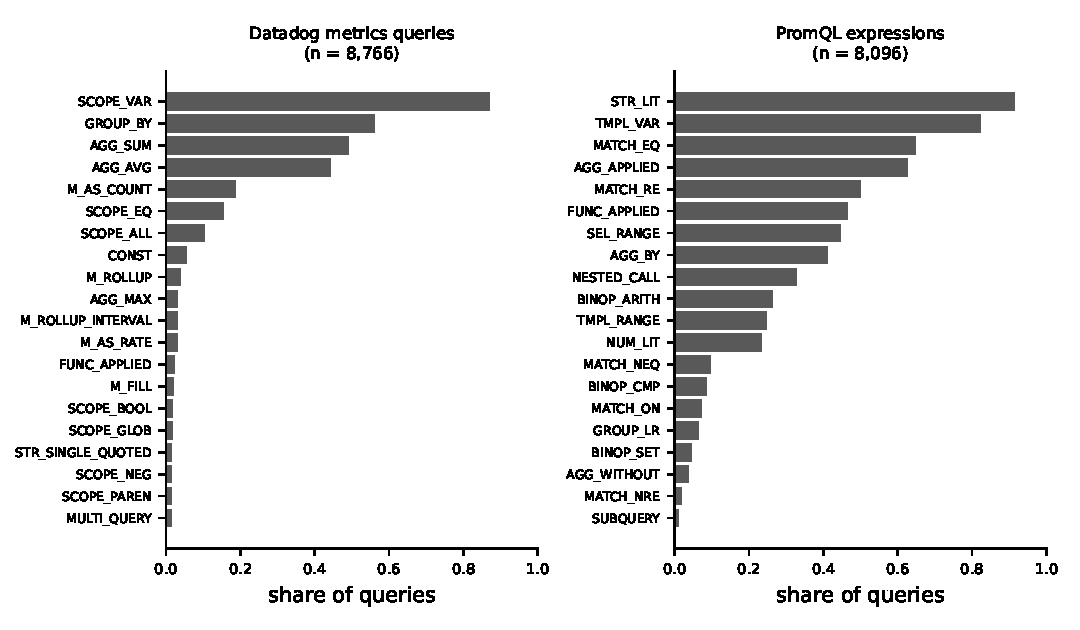
\includegraphics[width=\linewidth]{figures/feature_frequency}
\caption{The twenty most frequent structural features per language, as a share of
queries. Feature codes are those of \texttt{corpus.FEATURE\_DOC}; a query contributes to
every feature it uses.}
\label{fig:feature-frequency}
\end{figure}

\begin{table}[htbp]\centering\footnotesize
\begin{tabular}{@{}lllr@{}}
\toprule
Language & Kind & Name & Occurrences \\
\midrule
datadog & aggregator & \texttt{sum} & 4,480 \\
datadog & aggregator & \texttt{avg} & 4,057 \\
datadog & aggregator & \texttt{max} & 275 \\
datadog & aggregator & \texttt{count} & 58 \\
datadog & aggregator & \texttt{min} & 51 \\
datadog & aggregator & \texttt{p95} & 19 \\
datadog & function & \texttt{.as\_count} & 1,766 \\
datadog & function & \texttt{.rollup} & 331 \\
datadog & function & \texttt{.as\_rate} & 266 \\
datadog & function & \texttt{.fill} & 185 \\
datadog & function & \texttt{top} & 163 \\
datadog & function & \texttt{.weighted} & 70 \\
datadog & function & \texttt{per\_minute} & 27 \\
datadog & function & \texttt{per\_second} & 22 \\
datadog & function & \texttt{derivative} & 15 \\
datadog & function & \texttt{count} & 8 \\
promql & aggregator & \texttt{sum} & 4,718 \\
promql & aggregator & \texttt{max} & 718 \\
promql & aggregator & \texttt{avg} & 621 \\
promql & aggregator & \texttt{count} & 307 \\
promql & aggregator & \texttt{topk} & 230 \\
promql & aggregator & \texttt{min} & 84 \\
promql & function & \texttt{rate} & 2,541 \\
promql & function & \texttt{irate} & 1,078 \\
promql & function & \texttt{histogram\_quantile} & 507 \\
promql & function & \texttt{increase} & 328 \\
promql & function & \texttt{label\_replace} & 152 \\
promql & function & \texttt{vector} & 113 \\
promql & function & \texttt{sort\_desc} & 91 \\
promql & function & \texttt{label\_join} & 55 \\
promql & function & \texttt{time} & 50 \\
promql & function & \texttt{round} & 46 \\
\bottomrule
\end{tabular}

\caption{The six most frequent space aggregators and ten most frequent functions per
language, by occurrence. Datadog's \texttt{p}$NN$ percentile aggregators are five
distinct operators totalling $34$ occurrences, of which only \texttt{p95} reaches this
table.}
\label{tab:operator-frequency}
\end{table}

\noindent
Four things in these distributions are load-bearing for the rest of the paper.

\emph{Datadog's head is very short.} \texttt{sum:} and \texttt{avg:} are $95\%$ of all
every space-aggregator occurrence in Table~\ref{tab:operator-frequency}, and \texttt{by \{...\}} appears in $56\%$ of
queries. A translator that handles two aggregators and grouping already speaks most of
what the corpus says.

\emph{The counter rule that matters is the undivided one.} \texttt{.as\_count()} outnumbers
\texttt{.as\_rate()} by $6.6$ to one ($1{,}766$ against $266$). Both reduce to the same
cumulative difference by Proposition~\ref{prop:offset}, which is why that proposition,
rather than anything about \texttt{rate}, is the one that carries a migration.

\emph{PromQL's head is a rate.} \texttt{rate} and \texttt{irate} together are $69\%$ of
all $5{,}227$ function occurrences. Meanwhile subqueries appear in $1.1\%$ of PromQL
queries, \texttt{offset} in $0.3\%$, and the \texttt{@} modifier in none at all --- a
construct the language has and $8{,}096$ shipped expressions never reach for. The gap
between what a query language contains and what its users employ is itself part of the
switching-cost story: the hard parts of a language can be rare.

\emph{Nothing is used alone.} A real Datadog query combines a space aggregator, a scope
of several terms, a grouping and at least one method. That is why marginal frequency is
the wrong order to build a translator in, and why the next subsection reports a different
order.

